\documentclass[a4paper, 12pt]{article}

\usepackage[portuges]{babel}
\usepackage[utf8]{inputenc}
\usepackage{amsmath}
\usepackage{indentfirst}
\usepackage{graphicx}
\usepackage{multicol,lipsum}

\begin{document}
%\maketitle

\begin{titlepage}
	\begin{center}
	
	%\begin{figure}[!ht]
	%\centering
	%\includegraphics[width=2cm]{c:/ufba.jpg}
	%\end{figure}

		\Huge{Universidade Estadual de Campinas - Unicamp}\\
		\large{IMECC}\\ 
		\large{MS571 - Aprendizado Máquinas : Aspectos T. e Práticos}\\ 
		\vspace{15pt}
        \vspace{95pt}
        \textbf{\LARGE{Projeto Computacional I }}\\
		%\title{{\large{Título}}}
		\vspace{3,5cm}
	\end{center}
	
	\begin{flushleft}
		\begin{tabbing}
			Matheus Feres Turcheti 241727\\
            Othavio Henrique de Jesus Ayres 246666\\
            Ricardo Raimundo da Silva 120094\\
	\end{tabbing}
 \end{flushleft}
	\vspace{1cm}
	
	\begin{center}
		\vspace{\fill}
			 Outubro\\
		 2022
			\end{center}
\end{titlepage}
%%%%%%%%%%%%%%%%%%%%%%%%%%%%%%%%%%%%%%%%%%%%%%%%%%%%%%%%%%%

% % % % % % % % %FOLHA DE ROSTO % % % % % % % % % %

% % % % % % % % % % % % % % % % % % % % % % % % % %
\newpage
\tableofcontents
\thispagestyle{empty}

\newpage
\pagenumbering{arabic}
% % % % % % % % % % % % % % % % % % % % % % % % % % %
\section{Implementação da Rede neural}
Para implementação da rede neural utilizamos como fonte de consulta, principalmente, os slides e as notas de aula. Ao inicio da implementação tínhamos uma rede neural construída pelo professor e apresentada em aula para utilizar como esqueleto. Todavia esta rede neural não funcionava para um numero qualquer de camadas escondidas e de neurônios. A ideia aplicada foi salvar cada um dos elementos da rede neural, em uma lista que poderia conter uma quantidade qualquer daquele elemento. Por exemplo, para as ativações, criamos uma lista $a$, na qual cada um de seus elementos é uma matriz de ativação cujo ínidce na lista corresponde à camada a que pertence. Ainda assim,  guardar os dados em listas não foi suficiente, pois como as funções  foram construídas para uma única camada escondida, algumas das funções tiveram que ser alteradas e outras criadas, a fim de realizar novos procedimentos além daqueles prontos. Como o cálculo do erro nos neurônios não é realizado para o \textit{bias}, a função \textit{gradientDescent} foi alterada para que não considerasse o bias da camada $i$, ao calcular o bias da camada $i-1$, desta forma a função passou a função a funcionar para um número qualquer de camadas escondidas, as quais, por sua vez, podem possuir um número qualquer de neurônios.

\section{Checagem de Gradiente}
O intuito deste algoritmo é realizar uma comparação entre os valores obtido pelo \textit{backpropagation} e a derivada numérica da função de custo $J$. Sua implementação foi bastante simples pois se tratava de um exercício conceitual, calculamos a derivada numérica pelo método da secante, utilizando um $\epsilon = 10^{-4}$ e, posteriormente, $\epsilon = 10^{-7}$. Em ambos os casos, obtivemos um erro médio (i.e. a diferença, em valor absoluto, entre cada gradiente do backpropagation o os valores obtidos pelo método da secante dividida pelo número total de neurônios da rede $N$) menor do que $\epsilon$ utilizado. Este método equivale a verificar que a norma 1 do vetor diferença entre os gradientes é inferior ao próprio $\epsilon \cdot N$; como há equivalência entre normas, é de se esperar que o resultado do algoritmo seja o mesmo, independente da escolha da norma.

\section{Representação Visual dos Thetas}
Nota-se que como demonstrado no artigo \cite{voss2021visualizing} existem diversas formas de vizualizar os pesos para problemas que envolvem previsões utilizando imagens. A função que desenvolvemos é pesadamente inspirada num \textit{snippet} encontrado ao pesquisar modos de fazer a visualização dos \textit{tethas} mais interessante \cite{Snaped}, e, como resultado, obtivemos uma imagem para unidade de ativação na primeira camada escondida, formadas ao reconstruir a matriz $20\times20$ a partir de cada linha da matriz de pesos $\Theta^{(1)}$. Esta imagem é uma representação de um "filtro" pois diz respeito a qual forma ou região da figura esta sendo analisada. Ou seja, conclui-se que os pesos dizem respeito ao que aquele neurônio está extraindo de uma imagem dada, e, por consequência, a ativação do neurônio a qual estas \textit{features} estão conectadas será um valor que representa o quanto da forma está contida na imagem original.

\section{Seleção de modelo}
Para realização desta etapa, foi desenvolvido um algoritmo que divide o conjunto total de exemplos de treino, em um conjunto de treino, um de validação e outro de testes. Nota-se que os elementos para todos os conjuntos são escolhidos de maneira aleatória pois caso contrário poderíamos poderíamos ter um conjunto enviesado e também que os testes foram realizados sobre a arquitetura com uma camada escondida que possui vinte e cinco neurônios (arquitetura original), pois o aumento de camadas e de neurônios não resultou em um aumento significativo de acurácia.
\begin{figure}[htb]
    \centering
    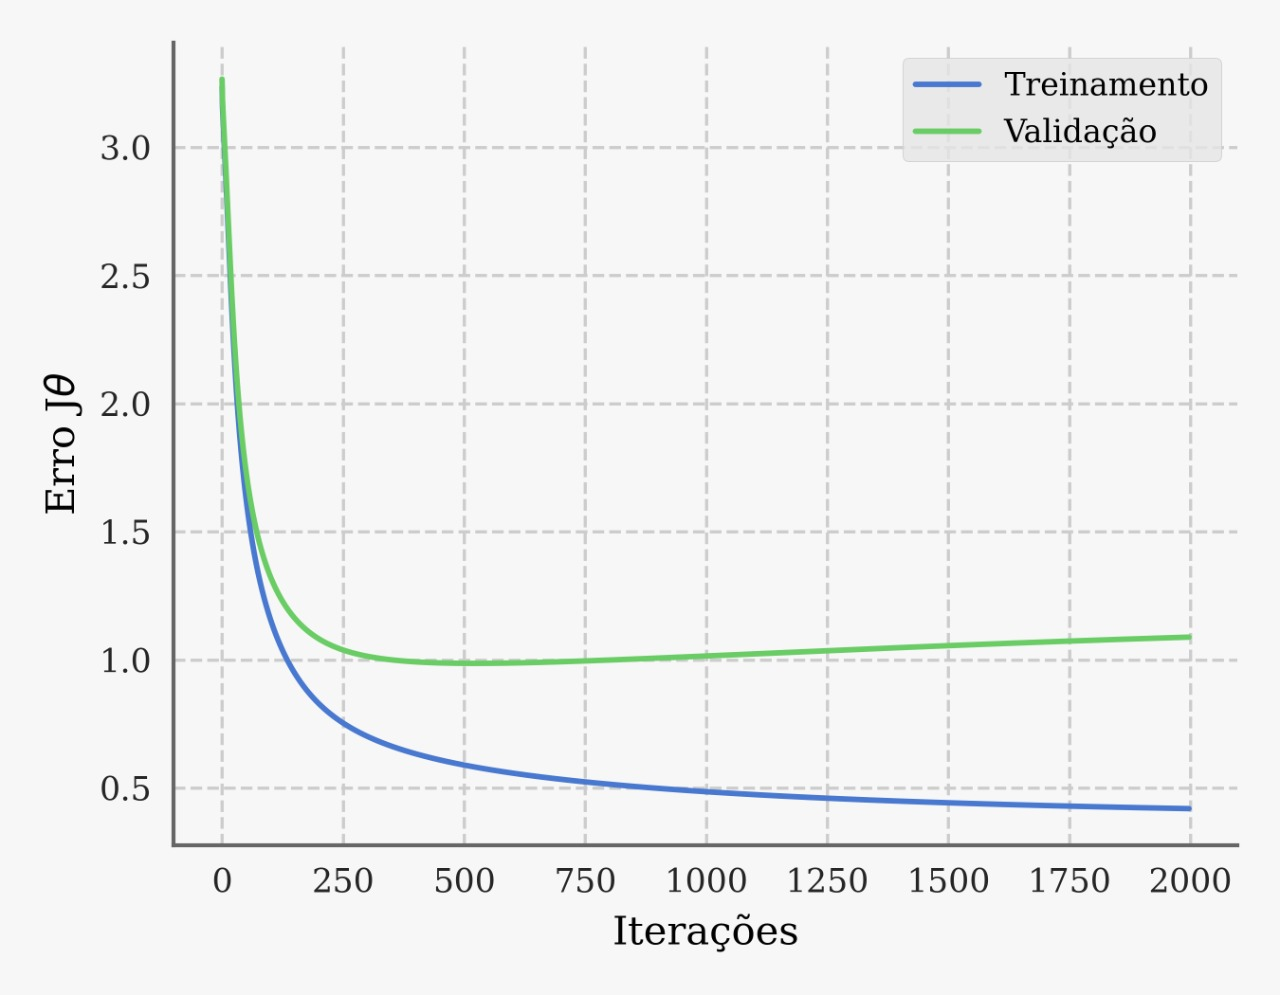
\includegraphics[width=0.8\linewidth]{graficos/erro_lambda1.png}
    \caption{Função de erro calculada para $\lambda $ igual a 1.}
    \label{fig:custo1}
\end{figure}
\subsection{Seleção dos lambdas}
Para se obter o melhor valor de lambda, realizamos o cálculo do erro para uma quantidade fixa de iterações, desta forma escolhemos o lambda ideal como aquele que mais reduz a função de custo.
\begin{figure}[htb]
    \centering
    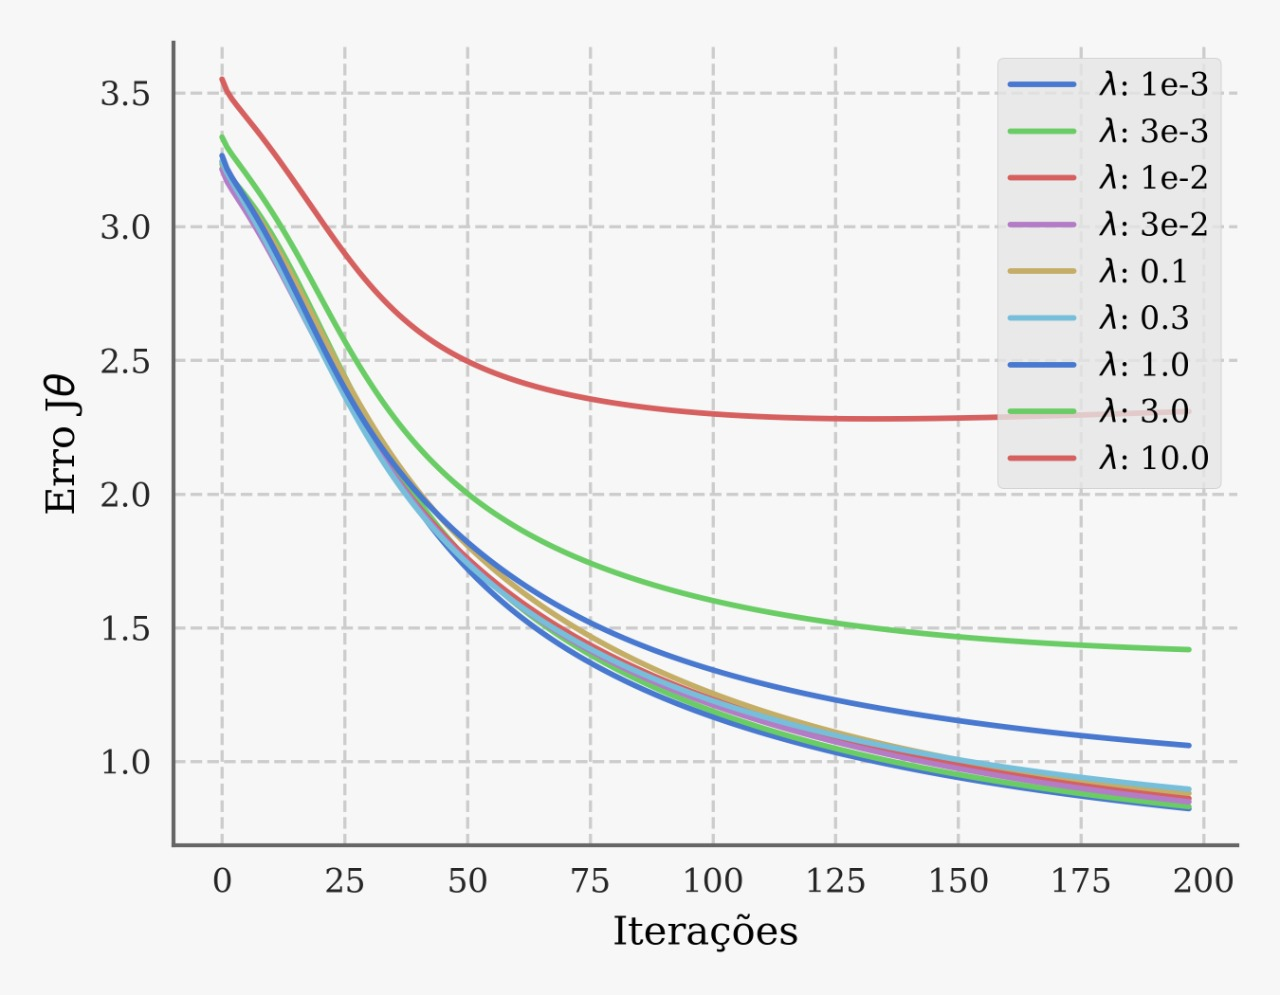
\includegraphics[width=0.60\linewidth]{graficos/teste_lambda.png}
    \caption{Testes realizados para escolha de $\lambda$.}
    \label{fig:lambda}
\end{figure}

Nota-se que que o valor com maior eficiência, ou seja, aquele que mais reduziu o custo foi $ \lambda $ igual a 0.001 como mostra a figura \ref{fig:zoom}
\begin{figure}[htb]
    \centering
    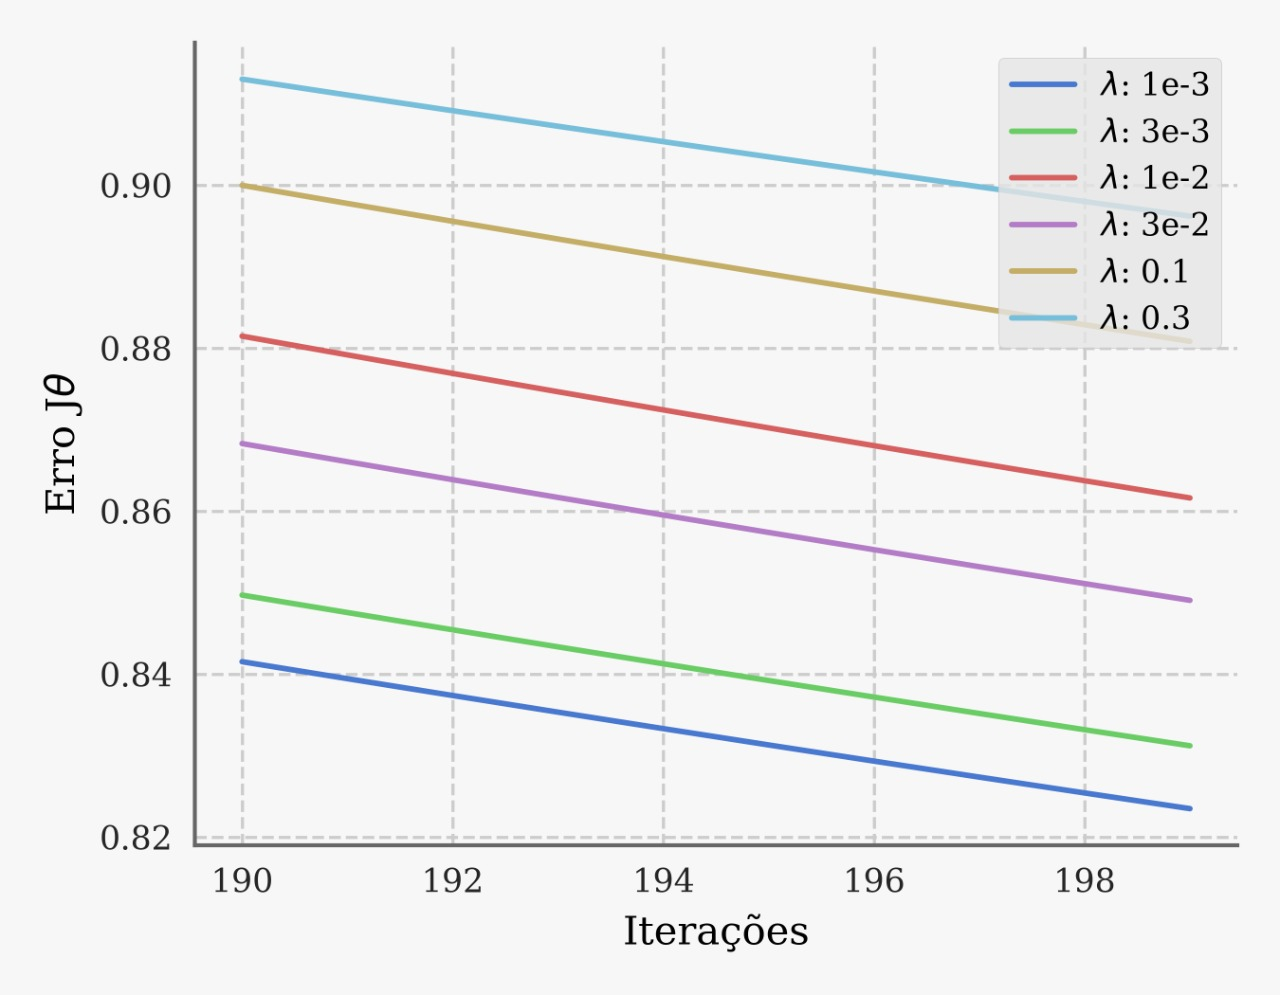
\includegraphics[width=0.64\linewidth]{graficos/zoom.png}
    \caption{Testes realizados para escolha de $\lambda$.}
    \label{fig:zoom}
\end{figure}
\newpage
Portanto, ao calcularmos novamente o grafico que representa o erro de validação, mas desta vez com o lambda otimizado temos o seguinte gráfico:
\begin{figure}[htb]
    \centering
    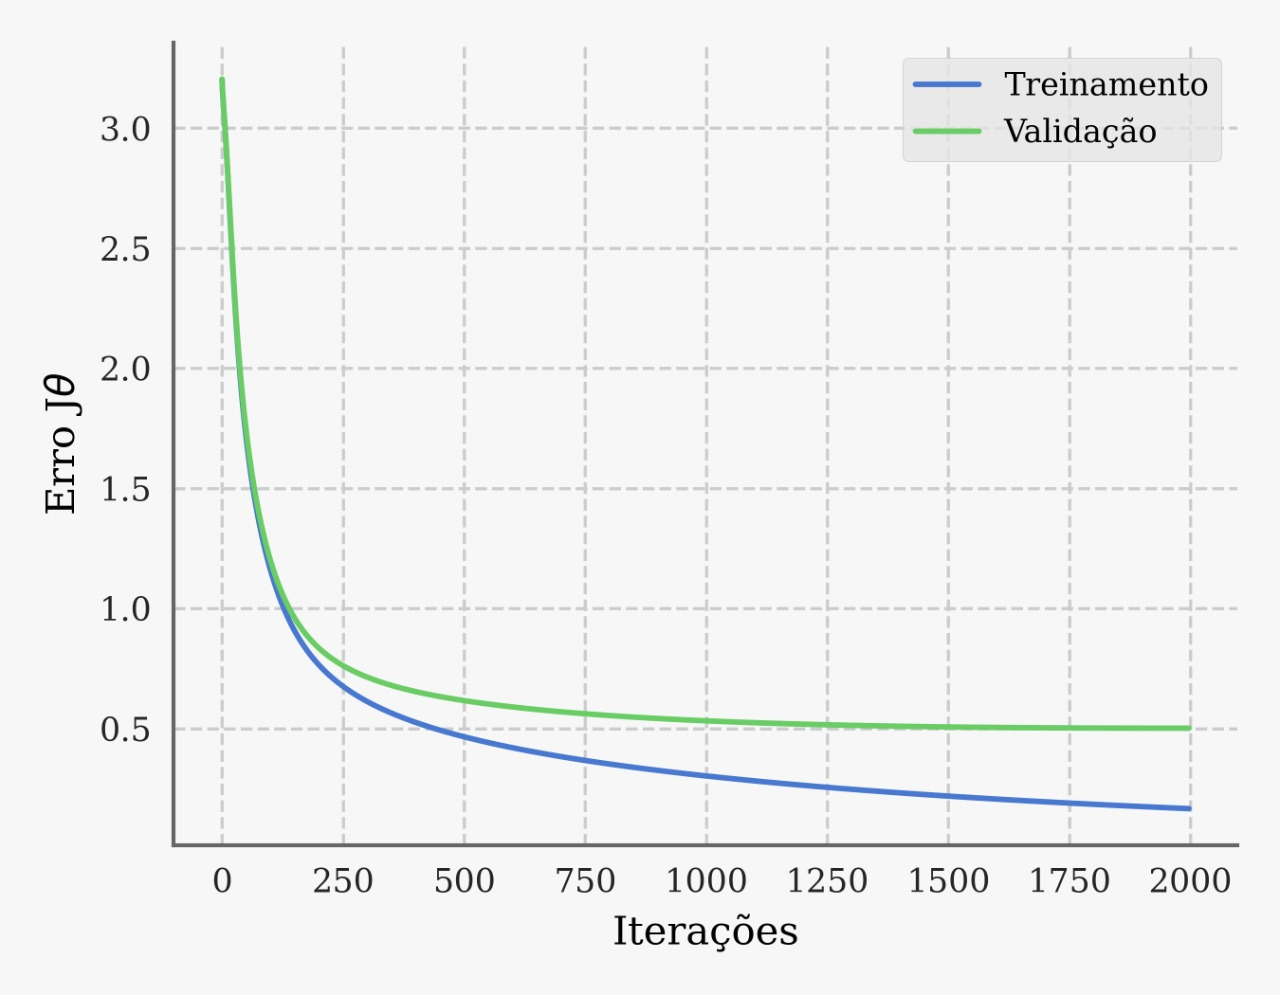
\includegraphics[width=0.8\linewidth]{graficos/erro_lambda_great.png}
    \caption{Testes realizados com $\lambda $ otimizado.}
    \label{fig:otimizado}
\end{figure}

É visível pela figura \ref{fig:otimizado} que a partir de uma certa 
quantidade de iterações a função de custo para o conjunto de validação 
atinge uma assíntota $h(x)$ igual a uma constante (neste caso 0.5) portanto mesmo que o treinamento 
siga diminuindo lentamente a validação não segue a mesma tendência.

Por fim, obtemos uma acurácia no conjunto de testes igual a 92.30\% utilizando de uma arquitetura com uma camada escondida que possui 25 neurônios, com taxa de aprendizado $\alpha$ igual a 1  e $\lambda$ igual a 0.001.



% --------------------------------------------------------
% REFERÊNCIAS BIBLIOGRÁFICAS
% 
\newpage

\bibliographystyle{unsrt}
\nocite{*}
\bibliography{bibliography}

\end{document}



